\documentclass[a4paper,10pt]{article}
\usepackage[utf8]{inputenc}
\usepackage[T1]{fontenc}
\usepackage{lmodern}	
\usepackage[italian]{babel}

\usepackage{amsmath}
\usepackage{amsfonts}
\usepackage{amssymb}

\usepackage{graphicx}
\usepackage[dvipsnames]{xcolor}  %colori

\usepackage{pgf}
\usepackage{tikz}
\usetikzlibrary{arrows,shapes,snakes,automata,backgrounds,petri}	% Finite States Machine

\usepackage[left=2cm,right=2cm,top=2cm,bottom=2cm]{geometry}
\geometry{a4paper}
\setlength\marginparwidth{40pt}
\setlength\marginparsep{1pt}

\usepackage{verbatim}
\usepackage{lipsum}

\usepackage{booktabs}
\usepackage{subfig}
\usepackage{float}
\usepackage{wrapfig}

\usepackage[colorlinks=true, linkcolor=black, urlcolor=blue, citecolor=darkgray, filecolor=darkgray]{hyperref}   %per gli hyperlink
\usepackage[italian, sort, noabbrev, capitalise]{cleveref}
\usepackage[bottom]{footmisc}

\usepackage[cdot, thickqspace, squaren]{SIunits}
% macro
\def\code#1{\texttt{#1}}

\title{Esercitazione 15: Misura della costante di Boltzmann attraverso misure di rumore}
\author{Gruppo BL \\ Candido Alessandro, Luzio Andrea, Mazziotti Fabrizio}

\begin{document}

\maketitle

\section{Scopo e Strumentazione}
In questa esercitazione si vuole effettuare una misura della costante di Boltzmann attraverso la
misura del rumore termico in una serie di resistenze con valori diversi.

\noindent La strumentazione è quella solitamente presente sul banco di lavoro, e inoltre si è usato:
\begin{itemize}
	\item INA114: Precision instrumentation amplifier;
	\item AD708: ultra low offset dual op-amp (2 integrati);
	\item AD736: true rms-to-dc converter.
\end{itemize}

\subsubsection*{Schema complessivo}

Lo schema a blocchi del circuito è riportato in \cref{fig:blocks}.

\begin{figure}[H]
	\centering
%	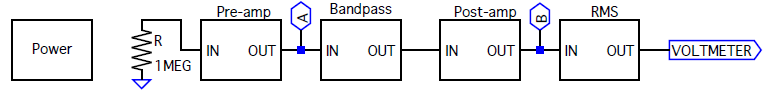
\includegraphics[width=\textwidth]{../grafici/Blocks.png}
	\vspace*{10pt}
	\caption{Schema a blocchi del circuito complessivo.}
	\label{fig:blocks}
\end{figure}

\section{Implementazione dei blocchi di circuito}

\subsection{Pre-amplificatore}

\begin{figure}[H]
	\centering
	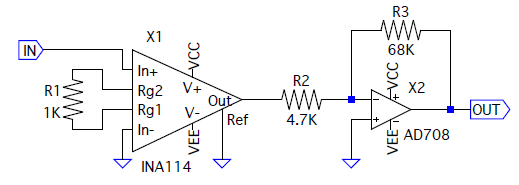
\includegraphics[width=\textwidth]{../grafici/preamp.png}
	\vspace*{10pt}
	\caption{Schema del Preamplificatore.}
	\label{fig:preamp}
\end{figure}


Si è montato il circuito in \cref{fig:preamp} costituito da due amplificatori: il primo è l'integrato INA114 il cui guadagno atteso è pari a $A_0 = (1+ 50k\Pmega/R_1) = 51.6 \pm 0.5$; %, dove la resistenza da 50 k$\Omega$ è il stata presa nominale poichè risultato delle resistenze interne all'integrato.


% la resistenza da 1k l'abbiamo misurata, quella da 50k sarà il risultato delle resistenze che stanno dentro all'integrato, che mettiamo nominale?

 il secondo è costituito da un opamp con feedback sull'ingresso invertente. Il guadagno atteso di questa seconda parte di circuito è dato da $A_1 = R_3/R_2 = 14.4 \pm 0.2 $.
Le resistenze utilizzate sono riportate in \cref{tab:resistenze}.

\begin{table}[H]
	\centering
	\begin{tabular}{ccc}
		\hline
		$R_1[\Omega]$ & $R_2[k\Omega]$ & $R_3[k\Omega]$\\
		\hline
		$989\pm9$ & $4.71\pm0.05$ & $67.9\pm0.6$\\
		\hline
	\end{tabular}
	\caption{Resistenze utilizzate nel circuito in \cref{fig:preamp}.}
	\label{tab:resistenze}
\end{table}

In primo luogo si è misurata la risposta in frequenza del solo amplificatore INA staccando la seconda parte del circuito e mandando al suo ingresso un'onda sinusoidale dal generatore di funzioni%con ampiezza picco-picco di $V_pp = 9.4\pm 0.2 mV$.
TABELLA FORSE?
FIT + IMMAGINE
Dal fit si ottengono come risultati $A_0 = $, $f_t,0 = $, $\chi^2/DOF = /$. Il guadagno è in buon accordo con quanto atteso. 
CHI2

In secondo luogo si è mandata un'onda sinusoidale all'ingresso della seconda parte del circuito (prima della resistenza $R_2$) e si è studiata la sua risposta in frequenza.
TABELLA FORSE?
FIT + IMMAGINE
Dal fit si ottengono come risultati $A_1 = $, $f_t,1 = $, $\chi^2/DOF = /$. Il guadagno è in buon accordo con quanto atteso. 

Inoltre affinché il circuito amplifichi il segnale al massimo possibile (quindi con l'amplificazione ricavata), è necessario che le frequenze di taglio ottenute nei due casi risultino maggiori della frequenza di risonanza del filtro passabanda (vedi prossima sezione), che è attesa essere $\sim$ 6-7 kHz. In entrambi i casi ciò è rispettato.




\subsection{Filtro passabanda e post amplificatore}

\subsection{Convertitore RMS}

\section{Misura della costante di Boltzmann} 

\subsection{Stima diretta dell'amplificazione \\e risposta in frequenza del circuito complessivo}

\subsection{Risultati finali}

\end{document}